\scanpage{35}
Posant
\[
\unsure{\xi|\zeta}^*_{E_y}(t)=t^{\chi^*(E_y)/2}L^*_{E_y}(t)
\]
on trouve
\[
\boxed{\unsure{\xi|\zeta}^*_{E_y}\left(\frac1{qt}\right)=\varepsilon'{}^*(E_y)\unsure{\xi|\zeta}^*_{E_y}(t)}
\]
\[
\left\{\begin{aligned}
\varepsilon'{}^*(E_y)&=\delta^*(E_y)q^{-\chi^*(E_y)/2}(-1)^{\chi^*(E_y)}\\
q&=p^{1+\rho}
\end{aligned}\right.
\]
\unsure{ceci avec les}

\uline{Un reproche à faire à} $L^*_{E_y}(t)$ : \uline{ce n'est pas} \uline{additif} en $E$. De façon précise, si on a
\diagram{\begin{tikzcd}[ampersand replacement=\&]0\arrow[r]\&E'_y\arrow[r,dash]\&E_y\arrow[r,dash]\&E''_y\arrow[r,dash]\&0\end{tikzcd}}
On en conclut
\diagram{\begin{tikzcd}[ampersand replacement=\&]0\arrow[r,dash]\&i_*(E'_y)\arrow[r,dash]\&i_*(E_y)\arrow[r]\&\unsure{i_y^*|i_*}(E''_y)\arrow[r]\&Q\arrow[r]\&0\end{tikzcd}}
où
\figure{\begin{tikzpicture}[x=1cm,y=1cm]
\node[anchor=west] at (0,1.6) {$Q\deleted{=\operatorname{Ker}\bigl(R^1i_*(E'_y)-R^1i_*(E_y)\bigr)}$};
\node[anchor=west] at (.5,.15) {$\inserted{=\coprod_{\substack{x\ \text{pt ramifié}\\\text{de }E''_y}}\unsure{j_x\longleftarrow X}}$};
\draw (.7,1.3) .. controls (.7,.8) and (1,.6) .. (.7,.5) .. controls (.2,.4) and (.4,-.8) .. (1.2,-.85) -- (3.5,-.7) .. controls (4.6,-.6) and (4.7,-.15) .. (4.3,.2) -- (7.8,.3) .. controls (8.8,.4) and (8.7,.9) .. (9,1.6);
\draw (8.7,1.65) .. controls (8.1,1.9) and (8,1.2) .. (7.7,1.35) .. controls (6.8,1.9) and (6.1,.35) .. (5.5,.4) .. controls (4.7,.7) and (5.3,1.6) .. (4.7,1.25) .. controls (3.5,.1) and (3.1,.05) .. (2.7,.7);
\end{tikzpicture}}
est concentré \deleted{\unsure{aux}} \unsure{en un nb} fini de pts de ``ramification'' de $E''_y$.

D'où
\[
\left\{\begin{aligned}
L^*_{E_y}(t)&=L^*_{E'_y}(t)L^*_{E''_y}(t)L_Q(t)^{-1}=L^*_{E'_y}(t)L^*_{E''_y}(t)\prod_xP_{Q_x}(t)\\
Q_x&=\operatorname{Coker}(E_x-E''_x)
\end{aligned}\right.
\]
\margin{\figure{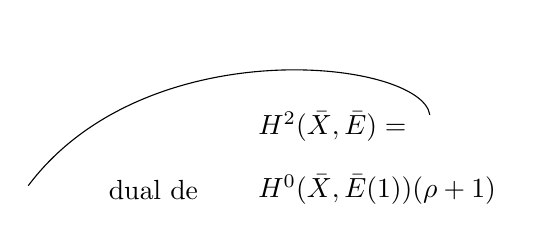
\begin{tikzpicture}[x=1cm,y=1cm]\draw (0,0) .. controls (1.5,2) and (5,1.6) .. (5.1,.9);\node[anchor=west] at (2.8,.75) {$H^2(\bar X,\bar E)=$};\node[anchor=west] at (.9,-.05) {dual de};\node[anchor=west] at (2.8,-.05) {$H^0(\bar X,\bar E\deleted{\unsure{(1)}})(\unsure{\rho+1})$};\end{tikzpicture}}}
\mspage{34}
